\section{Polarisation Spectroscopy}%\label{chapter:pol_spec}
\label{section:pol_spec_theory}

In \gls{ps} a circularly polarised pump beam from a monochromatic laser, with frequency close to an atomic resonance, induces frequency-dependent circular birefringence in a magnetically-shielded atomic gas sample.
A linearly polarised beam from the same laser source is used to measure the birefringence, monitored with a balanced polarimeter consisting of a half-wave phase retarder, \gls{pbs} and two detectors.
This is shown in Figure \ref{figure:pol_spec_schematic}.

\begin{figure}
\centering
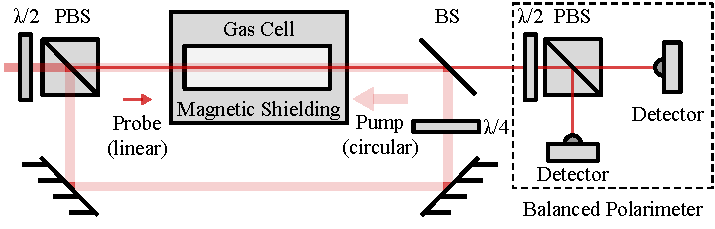
\includegraphics[width=\linewidth]{part1/Figs/PolSpecSchematic.pdf}
\caption{A schematic of \gls{ps} with a balanced polarimeter.
The power balance between the probe and the pump beam is controlled with the left-most $\lambda/2$ phase retarder and \gls{pbs}.
The $\lambda/4$ retarder is adjusted to produce a circularly polarised pump beam.
The non-polarising beamsplitter (BS) is used to counter-propagate the pump beam through the atomic sample without altering the polarisation of the circular pump or linear probe.
The final $\lambda/2$ retarder, \gls{pbs} and the detectors form the balanced polarimeter that monitors the polarisation rotation of the probe.}
\label{figure:pol_spec_schematic}
\end{figure}

The circularly polarised pump beam induces circular birefringence in the atomic sample by partial optical pumping of the sample into one of the extreme hyperfine sublevels, $m_F=\pm F$, where $m_F$ labels the hyperfine sublevel and $F$ is the atomic angular momentum number.
This partial optical pumping, referred to here as the anisotropy of the medium, results in unequal absorption coefficients for each circular polarisation.
The linearly polarised probe beam can be decomposed into two equal and oppositely circularly polarised components which undergo different absorption due to the anisotropy, such that when recombined after passing through the atomic sample the probe beam becomes elliptically polarised with an angle different to that of the original linear polarisation.
This process is depicted in Figure \ref{figure:pol_spec_explanation}.

\begin{figure}
\centering
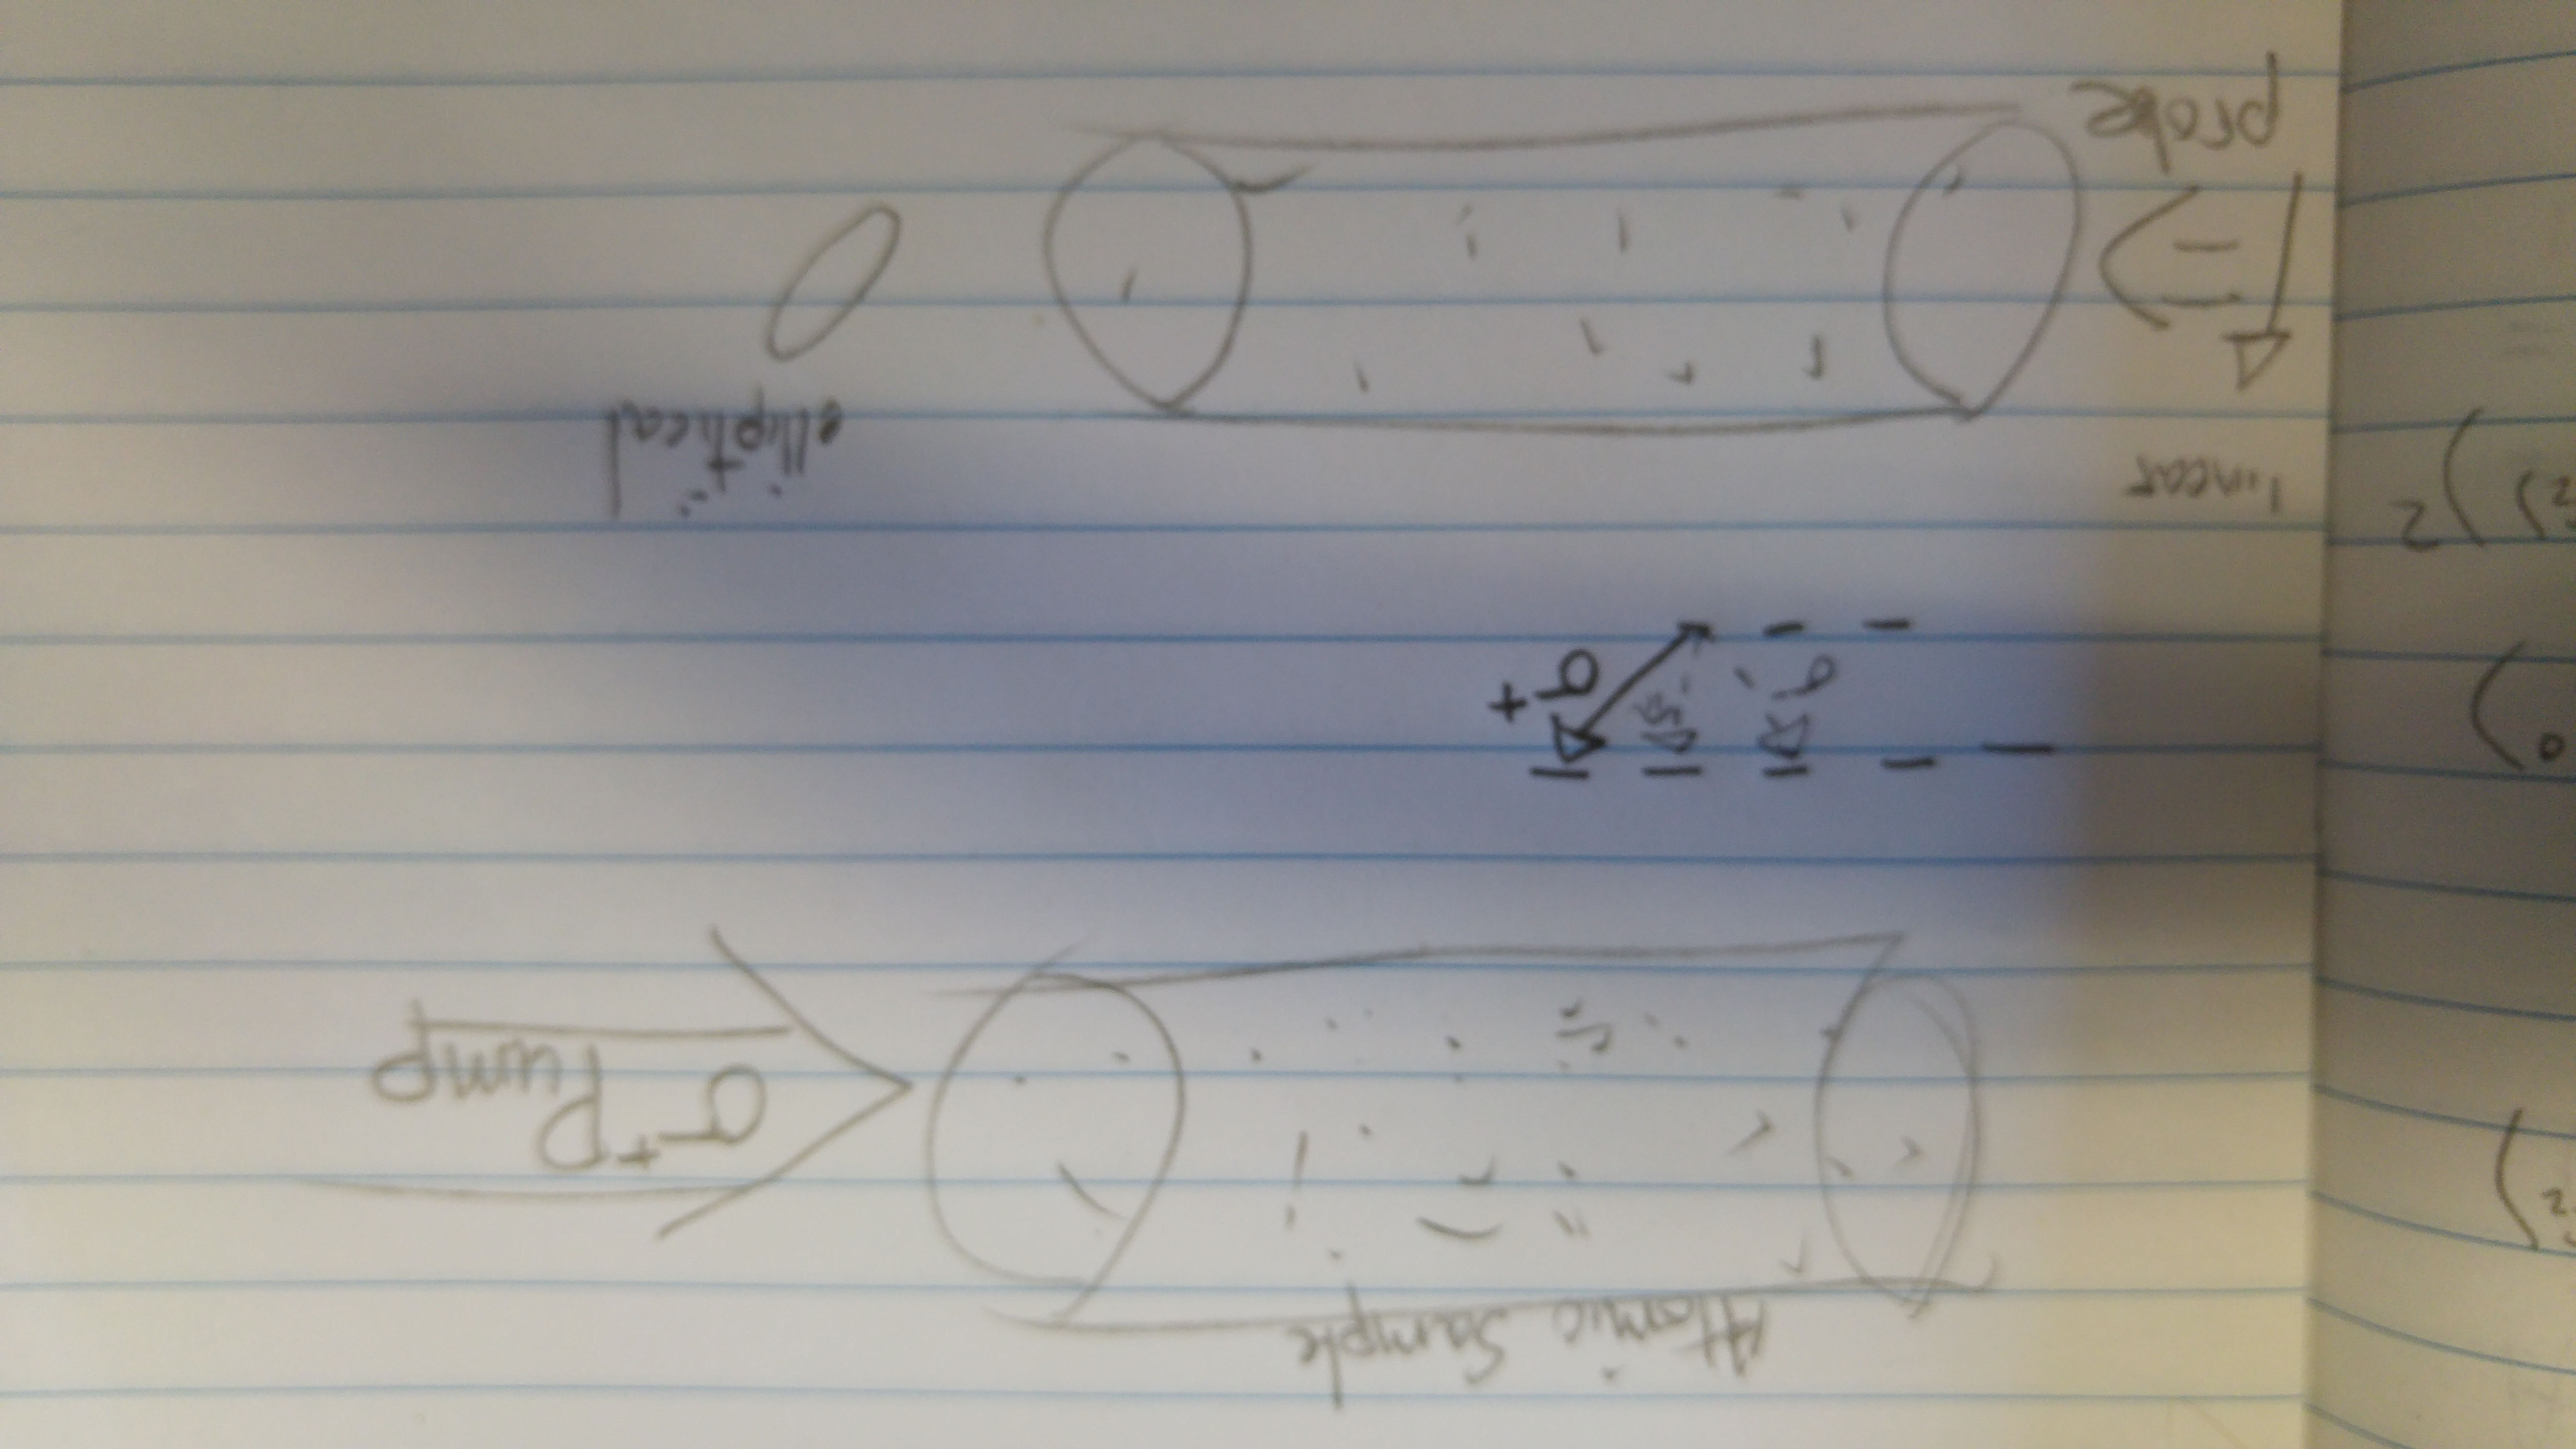
\includegraphics[width=\linewidth,angle=180]{part1/Figs/pol_spec_explanation_placeholder.jpg}
\caption{A conceptual figure for explaining the basics of pol spec.}
\label{figure:pol_spec_explanation}
\end{figure}

Consider the electric field of the probe beam before it enters the atomic sample at an angle $\phi$ to the $x$ axis:
\begin{equation}
\vec{E}=E_0\big(\cos{\phi}\,\hat{x}+\sin{\phi}\,\hat{y}\big)
\end{equation}
which can be expressed in terms of the circularly polarised basis vectors, $(\hat{x}\pm i\hat{y})$,
\begin{equation}
\vec{E} = \frac{E_0}{2}e^{-i\phi}(\hat{x}+i\hat{y}) + \frac{E_0}{2}e^{+i\phi}(\hat{x}-i\hat{y})
\end{equation}

After propagating through an atomic sample of length $L$ with refractive indices for the circular polarisation components of $n_\pm$, and absorption coefficients of $\alpha_\pm$ the electric field becomes
\begin{align}
\vec{E}\  = \ &\frac{E_0}{2}e^{-i\phi}\,\exp\left[\frac{i\omega n_+ L}{c} - \frac{\alpha_+ L}{2}\right](\hat{x}+i\hat{y})\quad +\quad \frac{E_0}{2}e^{+i\phi}\,\exp\left[\frac{i\omega n_- L}{c} - \frac{\alpha_- L}{2}\right](\hat{x}-i\hat{y}) \notag\\ 
\  = \ &\frac{E_0}{2} e^{-i\phi}\,\exp\left[\frac{i\omega L}{2c}(n_+-n_-) + \frac{i\omega L}{2c}(n_+ + n_-) - \frac{L}{4}(\alpha_+ -\alpha_-) - \frac{L}{4}(\alpha_+ + \alpha_-)\right](\hat{x}+i\hat{y})\ +\notag\\
&\frac{E_0}{2} e^{+i\phi}\,\exp\left[-\frac{i\omega L}{2c}(n_+-n_-) + \frac{i\omega L}{2c}(n_-+n_+) + \frac{L}{4}(\alpha_+-\alpha_-) - \frac{L}{4}(\alpha_-+\alpha_+) \right](\hat{x}-i\hat{y}) \notag\\
\  = \ &\frac{E_0}{2} \exp\left[\frac{i\omega L}{2c}(n_+ + n_-) - \frac{L}{4}(\alpha_+ + \alpha_-)\right] \left\{ e^{-i(\phi - \Omega)}\, \, (\hat{x}+i\hat{y})\ + e^{+i(\phi-\Omega)}\,(\hat{x}-i\hat{y})\right\},\label{equation:elliptically_polarised}
\end{align}
where
\begin{equation}
\Omega = \frac{\omega L}{2c}(n_+-n_-) + i\frac{L}{4}(\alpha_+ -\alpha_-).
\end{equation}
Equation \ref{equation:elliptically_polarised} represents elliptically polarised light with the major axis at an angle of $\theta = \phi + \Omega$ to the $x$-axis.

The horizontal and vertical polarisation components of the beam are separated by the \gls{pbs},
\begin{align}
\vec{E} = &\frac{E_0}{2} \exp\left[\frac{i\omega L}{2c}(N_+ + n_-) - \frac{L}{4}(\alpha_++\alpha_-)\right]\ \left[ \hat{x} \left(e^{-i(\phi-\Omega)}+e^{-i(\phi-\Omega)}\right) + i\hat{y} \left(e^{-i(\phi-\Omega)}-e^{-i(\phi-\Omega)}\right)\right]\notag\\
 = & E_0 \exp\left[\frac{i\omega L}{2c}(N_+ + n_-) - \frac{L}{4}(\alpha_++\alpha_-)\right] \bigg[ \hat{x} \cos(\phi-\Omega) + \hat{y} \sin(\phi-\Omega)\bigg],
\end{align}
and the intensity of the beams are then detected by photodetectors,
\begin{align}
I_x &= |E_x|^2 \notag \\
& = \left|E_0 \exp\left[\frac{i\omega L}{2c}(N_+ + n_-) - \frac{L}{4}(\alpha_++\alpha_-)\right] \cos(\phi-\Omega) \right|^2 \notag \\
& = E_0^2\left| \exp\left[\frac{i\omega L}{2c}(N_+ + n_-)\right]\exp\left[-\frac{L}{4}(\alpha_++\alpha_-)\right] \right|^2 \cos\bigg(\phi-\Omega\bigg) \cos\bigg(\overline{\phi-\Omega}\bigg) \notag \\
& = E_0^2 \exp\left[-\frac{L}{2}(\alpha_++\alpha_-)\right] \cos\bigg(\phi-\frac{\omega L}{2c}(n_+-n_-) + i\frac{L}{4}(\alpha_+ -\alpha_-)\bigg) \cos\bigg(\phi-\frac{\omega L}{2c}(n_+-n_-) - i\frac{L}{4}(\alpha_+ -\alpha_-)\bigg) \notag \\
& = \frac{E_0^2}{2} \exp\left[-\frac{L}{2}(\alpha_++\alpha_-)\right] \left[\cos\bigg(2i\frac{L}{4}(\alpha_+ -\alpha_-)\bigg) + \cos\bigg(2\phi-2\frac{\omega L}{2c}(n_+-n_-)\bigg)\right] \\
\notag\\
I_y &= |E_y|^2 \notag \\
& = \left|E_0 \exp\left[\frac{i\omega L}{2c}(N_+ + n_-) - \frac{L}{4}(\alpha_++\alpha_-)\right] \sin(\phi-\Omega) \right|^2 \notag \\
& = \frac{E_0^2}{2} \exp\left[-\frac{L}{2}(\alpha_++\alpha_-)\right] \left[\cos\bigg(2i\frac{L}{4}(\alpha_+ -\alpha_-)\bigg) - \cos\bigg(2\phi-2\frac{\omega L}{2c}(n_+-n_-)\bigg)\right]
\end{align}
and subtracted by electronics to generate the error signal,
\begin{align}
\epsilon =\ &I_y - I_x = E_y^2 - E_x^2 \notag \\
=\ &E_0^2 \exp\left[-\frac{L}{2}(\alpha_++\alpha_-)\right] \cos\bigg(2\phi-2\frac{\omega L}{2c}(n_+-n_-)\bigg).
\end{align}

The spectral profile of $(\alpha_+-\alpha_-)$ is a power-broadened Lorentzian~\cite{pearman_polarization_2002},
\begin{equation}
\alpha_+ - \alpha_- = \frac{\Delta\alpha_0}{1+x^2},
\end{equation}
where $x=\frac{\omega_0-\omega}{\Gamma/2}$ is the detuning scaled by the atomic linewidth $\Gamma$, and $\Delta\alpha_0$ is the maximum difference in absorption coefficients at the atomic resonance.
The absorption cooefficients and refractive indices are related via the Kramers-Kronig dispersion relation~\cite{demtroder_laser_2014},
\begin{equation}
n_+ - n_- = \frac{c}{\omega_0} \Delta\alpha_0 \frac{x}{1+x^2}.
\end{equation}
Typically the polarisation rotation induced by the medium is small and is maximised when $\phi=\frac{\pi}{4}$ giving the approximate error signal,
\begin{equation}
\epsilon \simeq - I_0 e^{-L(\alpha_++\alpha_-)/2}\left( L \Delta\alpha_0 \frac{x}{1+x^2}\right)
\end{equation}

\Gls{ps} produces a dispersion shaped spectrum about the atomic resonance with zero background, as shown in {\color{red}PS SPECTRUM FIGURE}, and is ideal for laser locking due to the large capture range and steep gradient near the resonance.
Unlike \gls{pdh}, \gls{ps} acts as an absolute reference as it tied to the frequency of the atomic-ensemble reference rather than a cavity.



\subsubsection{Magnetic shielding}

\subsubsection{Balanced Polarimeter}

Balanced polarimeter.\cite{pearman_polarization_2002,yoshikawa_frequency_2003}

When Wieman and H\"anch~\cite{wieman_doppler-free_1976} originally described \gls{ps} polarisation rotation was monitored with a nearly crossed polariser as shown in Figure \ref{figure:wieman_doppler-free_schematic}.
The polariser is crossed such that only a small proportion of the probe beam passes through them in the absence of the pump.
With the pump inducing anisotropy the rotation of the probe can be detected after the polarisers.

\begin{figure}
\center
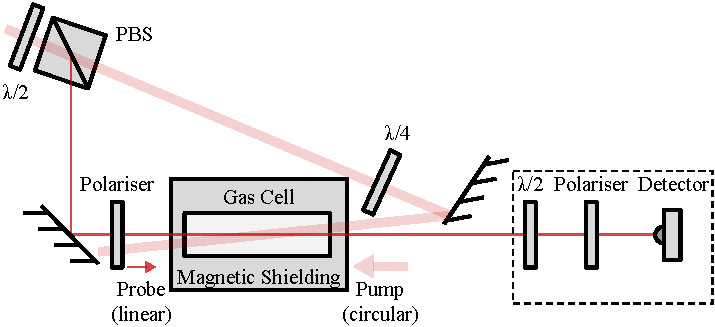
\includegraphics{part1/Figs/PolSpecWieman.pdf}
\caption{Caption.}
\label{figure:wieman_doppler-free_schematic}
\end{figure}

Pearson et al. proposed the alternative method of using a balanced polarimeter which provides a background-free signal with peak-to-peak height more than an order of magnitude greater than with the crossed polariser method~\cite{pearman_polarization_2002}.

\subsubsection{Co-propagating Beams}

All papers thus far have ``snuck'' the pump beam through the vapour cell.

Figure with ``snucked'' and beam splitter configuration.

The angle of ``snucking'' has implications that there is math for...

Using a NBPS instead means you have an angle of 0.
The beam splitter has no effect on the polarisation as far as I can tell.

Pumped spectroscopy techniques such as \gls{ps} and \gls{sa}... spectral broadening due to angle stuff.

\subsection{Fast Theory}

\subsection{Developments}

\subsubsection{High bandwidth feedback}


\subsubsection{Lincoln's magic detectors?}

\subsection{Experimental Setup (with details - fibres, calcite, etc.)}

